\begin{tabular}{ll}
    \toprule
    Input: &
    \begin{tabular}[t]{@{}l@{}}
        Spectrum $I=(I_\s{x}, \,I_\s{y})$ a $\lambda \times 2$ array\\
        $I_\s{x/y}$ ... X and Y-transmission spectra,
        $\lambda$ ... number of wavelengths
    \end{tabular}\\
    Output: & two sets layer parameters $p, \, m, \, g$ and stack parameters
    $\varphi, \, h$ \\
    \bottomrule
\end{tabular}

\paragraph{Network Architecture}
This module is a 1D Convolutional Neural Network instead of the simple Multi Layer Perceptron. It was chosen to utilize the translational invariance of ConvNets. For example the concept "peak" should be learned independent of its position in the spectrum. As described in section \ref{sec:NN_bg} a ConvNet provides this functionality. Another constraint on the network architecture arises from the different kind of outputs.
$p = (w, \, l, \, t, \, \Lambda), \, \varphi$ and $h$
are continuous and $m, \, g$ are discrete/categorical.
These need different activation functions $\sigma$ to reach the different value ranges. The continuous outputs are mostly bounded by physical constraints and $m, \, g \in [0, \, 1]$ as they are \textit{one hot encoded} meaning $1 \rightarrow$ "The layer has this property" and
$0 \rightarrow$ "The layer does not have this property".


The different outputs also need different cost functions $C(y, y')$ during training where $y'$ is the networks output and $y$ is the known solution. For the continuous output one can simply use the mean squared error

\begin{equation}
    C_\s{mse}(\vb y, \, \vb y') = \sum_i \qty(y_i - y_i')^2
\end{equation}

\noindent
as all outputs are equally important and the cost function should be indifferent on whether the networks prediction is over or under target. For the categorical output the network learns quicker with the \textit{Categorical Cross-Entropy} error.

\begin{equation}
    C_\s{ce}(\vb y, \, \vb y') = - \sum_i y_i \log y'_i,
\end{equation}

\noindent
Using this error if the network predicts $y'_i = 0$ for all categories then $C_\s{ce} \rightarrow \infty$. \note{why is this better?}

The final architecture is similar to the example given in figure \ref{fig:bg:NN_example} while meeting the above-mentioned constraints:

\begin{figure}[H]
    \centering
    \includegraphics[width=\linewidth]{al_NN_architecture}
    \caption{The network starts with 4 pairs of convolutional and pooling layers. The convolutions are characterized by (\textit{number of kernels}, \textit{kernel size}). The kernel size is always 5 and the number of kernels is gradually increased. Then the Network splits into a discrete and a continuous branch via two Dense layers with (\textit{number of neurons}). \note{Dropout missing}
    All the internal activations $\sigma_\s{r}$ are ReLu's and the final activations $\sigma_\s{s}$ and $\sigma_{l}$ are a sigmoid and a linear function.}
    \label{fig:al:NN_architecture}
\end{figure}

\newpage
\paragraph{Network Training}
To train a Neural Network one needs a training set $(X, \, Y)$ of known input output pairs. In this case they are generated using the pre simulated single layers in the Database which are randomly combined into a stacks. Then the input spectrum is calculated via SASA.
